\label{section_results}
We developed a code in Python based on the methods exposed in Section \ref{section_models_maze} for assessing our algorithm's performance. Pseudocode \ref{pseudocode_1} and Pseudocode \ref{pseudocode_2} guided the reasoning behind the code, that is available on \href{https://github.com/ArthurJose2000/mazeexploration}{github.com/ArthurJose2000/mazeexploration}.

This work used perfect mazes for simulating multi-agent scenarios where agents go through the mazes in order to find the goal. Section \ref{section_results_our_performance} presents the agents's performance when they use our algorithm. Section \ref{section_results_incremental_policy} proposes an agent policy modification when it finishes its interval for improving its performance. Finally Section \ref{section_results_tarry_vs_our} compares our algorithm's performance to the performance of the extended Tarry's algorithm \cite{KivelevitchCohen2010}, despite the latter having communication between agents.

\section{Our algorithm's perfomance}
\label{section_results_our_performance}

In order to assess our algotihm's performance, this work generates, using the code provided by \citen{Muhammad2021}, 250 random and perfect mazes for each type of size - $10 \times 10$, $20 \times 20$, $30 \times 30$, and $40 \times 40$. As they are perfect mazes, i.e., there is only one path to the goal from any cell, any node of the maze's tree representation has the same convergence interval for every agent. Thus, the developed code aims to fill the concept of dispersion, where the agents try to go through the maze as dispersed as possible without communication.

For each maze size, the code ran 1 single agent until 40 cooperative agents going through 250 different mazes, since this work generated 250 random perfect mazes for each type of size.....

\begin{figure}
\centering
\begin{subfigure}{.5\textwidth}
  \centering
  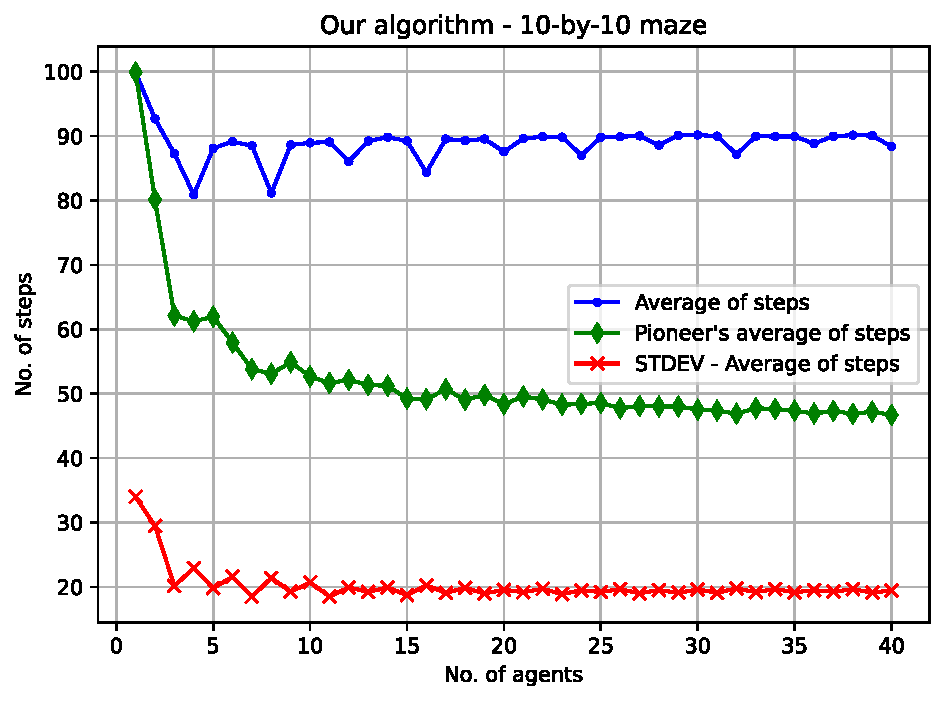
\includegraphics[width=.4\linewidth]{Cap3/our_algorithm/our_algorithm_10x10_steps.pdf}  
  \caption{Put your sub-caption here}
  \label{fig:sub-first}
\end{subfigure}
\begin{subfigure}{.5\textwidth}
  \centering
  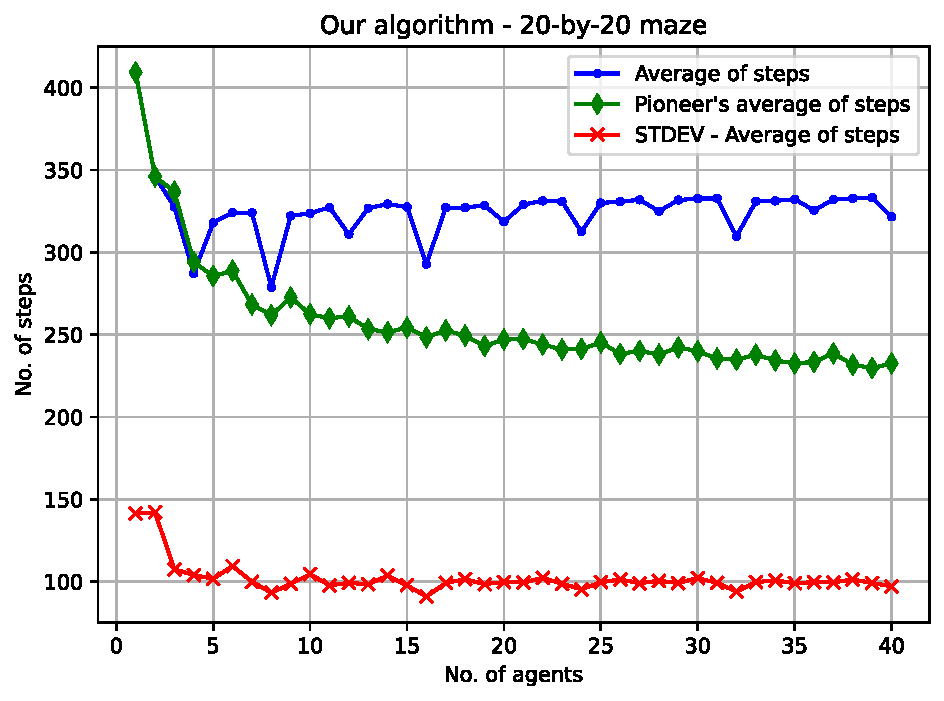
\includegraphics[width=.4\linewidth]{Cap3/our_algorithm/our_algorithm_20x20_steps.pdf}  
  \caption{Put your sub-caption here}
  \label{fig:sub-second}
\end{subfigure}

\newline

\begin{subfigure}{.5\textwidth}
  \centering
  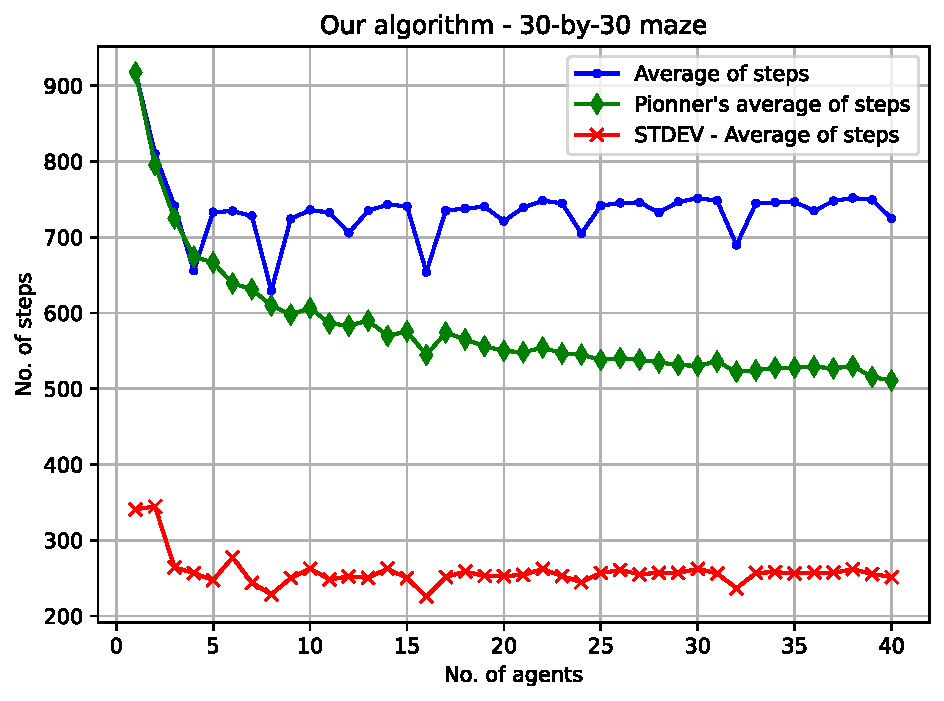
\includegraphics[width=.4\linewidth]{Cap3/our_algorithm/our_algorithm_30x30_steps.pdf}  
  \caption{Put your sub-caption here}
  \label{fig:sub-third}
\end{subfigure}
\begin{subfigure}{.5\textwidth}
  \centering
  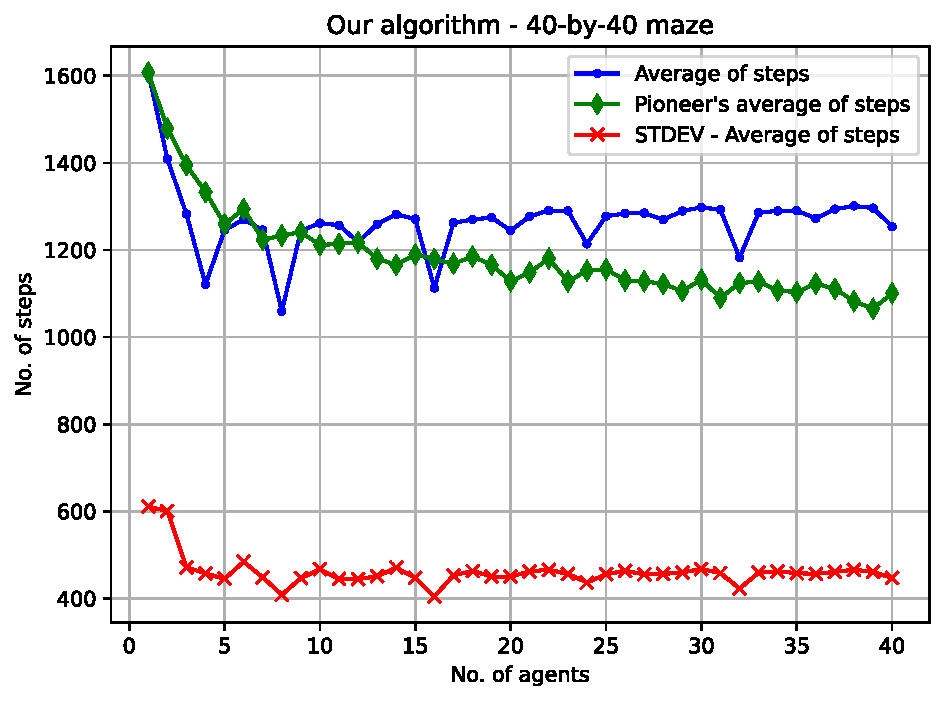
\includegraphics[width=.4\linewidth]{Cap3/our_algorithm/our_algorithm_40x40_steps.pdf}  
  \caption{Put your sub-caption here}
  \label{fig:sub-fourth}
\end{subfigure}
\caption{Put your caption here}
\label{fig:fig}
\end{figure}

\begin{figure}
    \centering
    \subfloat[\centering Agent at starting cell]
    {{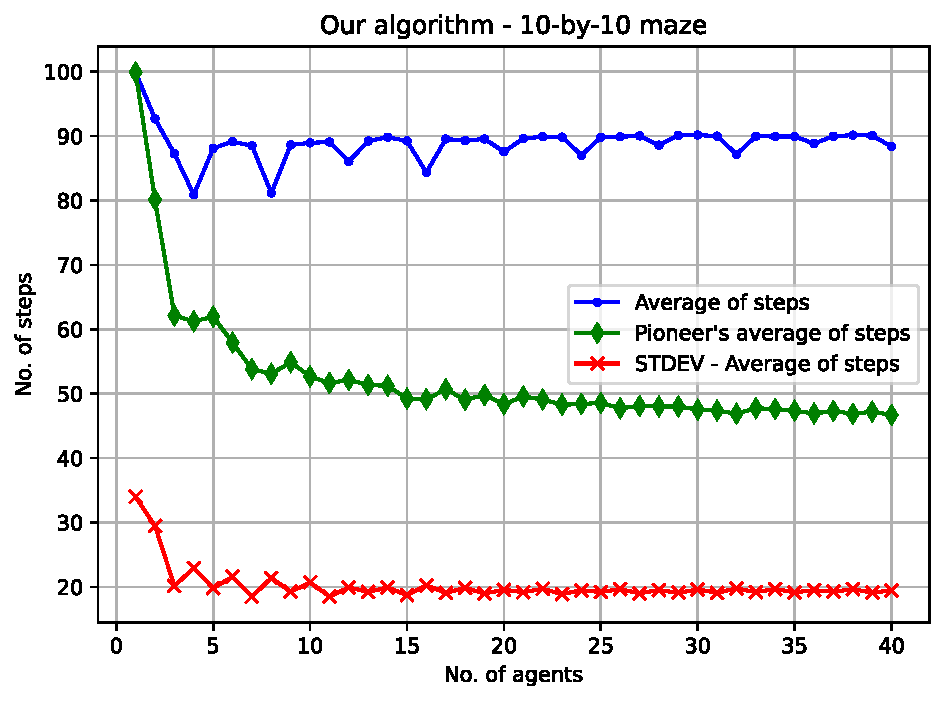
\includegraphics[width=3cm]{Cap3/our_algorithm/our_algorithm_10x10_steps.pdf} }}
    \qquad
    \subfloat[\centering Agent's 2nd step]
    {{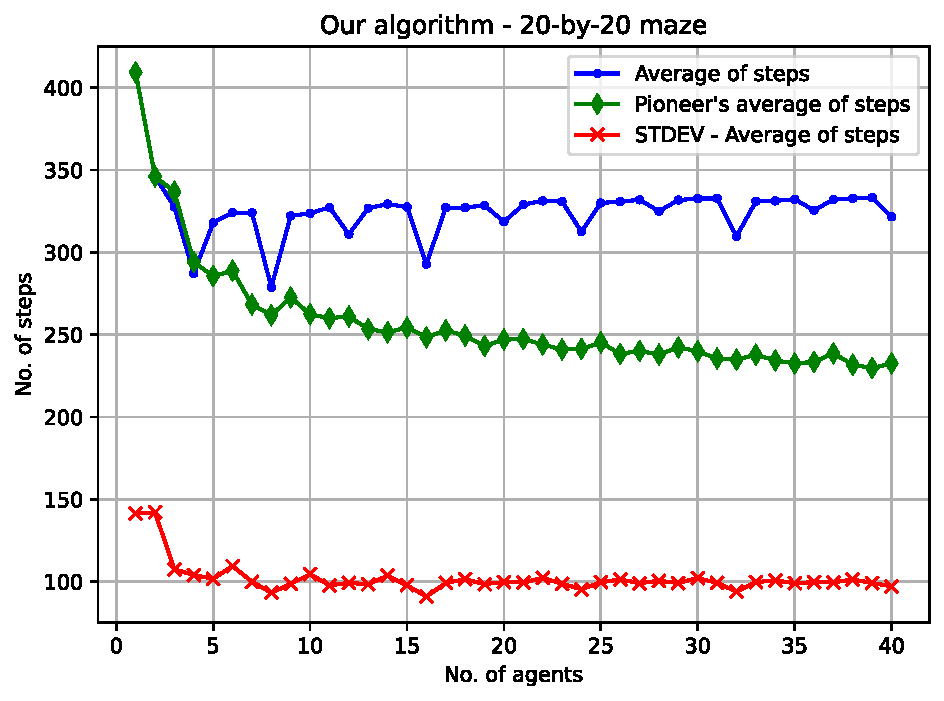
\includegraphics[width=3cm]{Cap3/our_algorithm/our_algorithm_20x20_steps.pdf} }}
    \qquad
    \subfloat[\centering Agent's 10th step]
    {{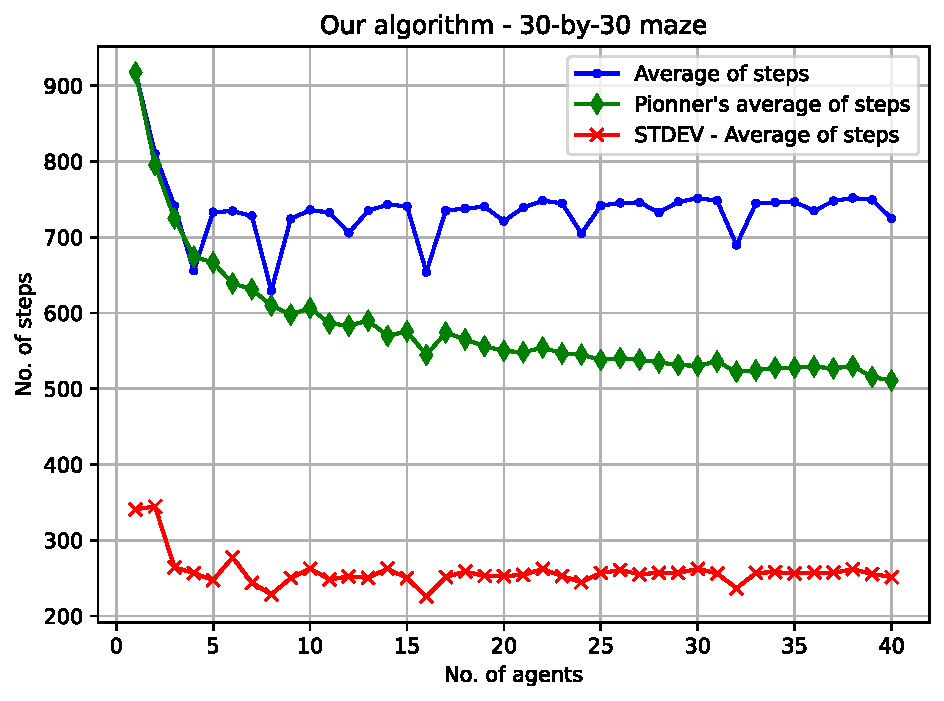
\includegraphics[width=3cm]{Cap3/our_algorithm/our_algorithm_30x30_steps.pdf} }}
    \newline
    \subfloat[\centering Agent's 10th step]
    {{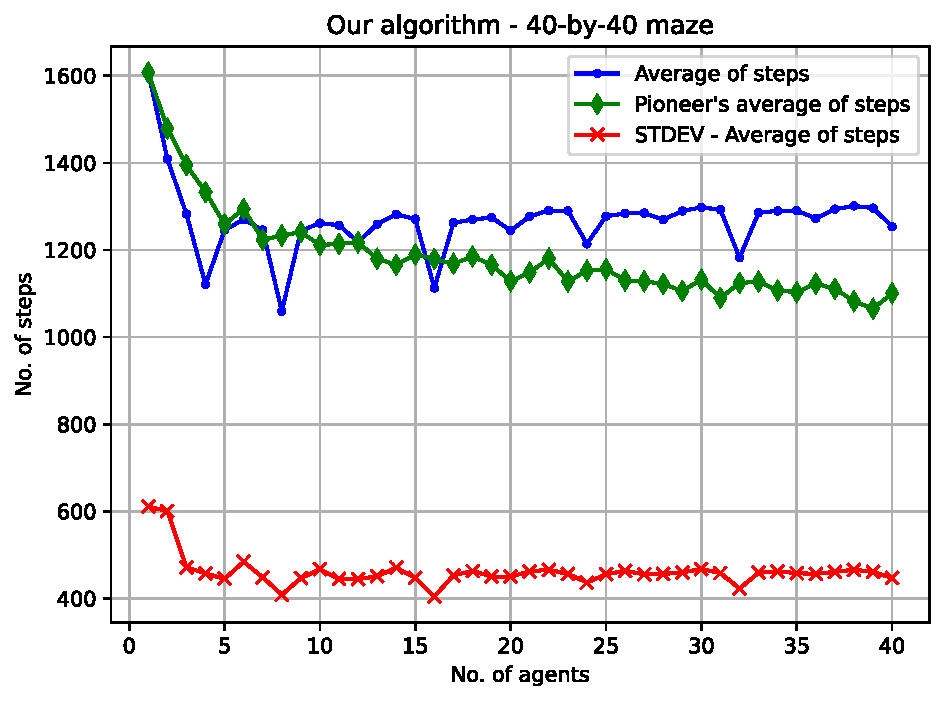
\includegraphics[width=3cm]{Cap3/our_algorithm/our_algorithm_40x40_steps.pdf} }}
    \caption{...}
    \label{maze_example}
\end{figure}



falar sobre a condição de parada 

\section{Incremental policy for the agents}
\label{section_results_incremental_policy}

\section{Our algorithm vs. Tarry's algorithm}
\label{section_results_tarry_vs_our}